\QCMautoevaluation{Pour chaque question, plusieurs réponses sont proposées. Déterminer celles qui sont correctes.}

\begin{QCM}
\begin{GroupeQCM}

\begin{exercice}
L'aire d'un disque de diamètre 6\,cm est de...
\begin{ChoixQCM}{4}
\item $6\pi$ cm\up{2}
\item $36$ cm\up{2}
\item $9\pi$ cm\up{2}
\item $36\pi$ cm\up{2}
\end{ChoixQCM}

\begin{corrige}
\reponseQCM{a}
\end{corrige}
\end{exercice}

\begin{EnonceCommunQCM}
Les questions \RefQCM{CDqcmA} à \RefQCM{CDqcmB} se réfèrent à la figure ci-dessous :
\end{EnonceCommunQCM}

\begin{center}
    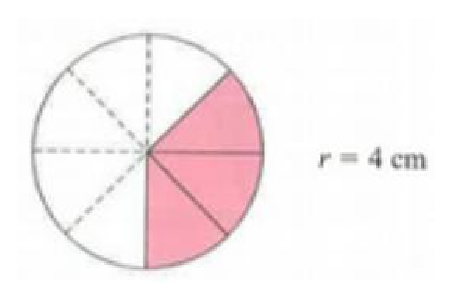
\includegraphics[width=.2\linewidth]{qcmCD01}
\end{center}

\begin{exercice}\label{CDqcmA}
L'aire du disque est :
\begin{ChoixQCM}{4}
\item $8\pi$ cm\up{2}
\item $4\pi^2$ cm\up{2}
\item $16\pi$ cm\up{2}
\item $16\pi$ cm
\end{ChoixQCM}

\begin{corrige}
\reponseQCM{a}
\end{corrige}
\end{exercice}



\begin{exercice}
L'aire du secteur angulaire rose (arrondie à 0,1 ) est :
\begin{ChoixQCM}{4}
\item $18,8$ cm\up{2}
\item $2,5$ cm\up{2}
\item $6,5$ cm\up{2}
\item $18,85$ cm\up{2}
\end{ChoixQCM}

\begin{corrige}
\reponseQCM{a}
\end{corrige}
\end{exercice}



\begin{exercice}\label{CDqcmB}
La circonférence du cercle est :

\begin{ChoixQCM}{4}
\item $8\pi$ cm
\item $4\pi^2$ cm
\item $16\pi$ cm
\item $8\pi$ cm\up{2}
\end{ChoixQCM}

\begin{corrige}
\reponseQCM{a}
\end{corrige}
\end{exercice}

\end{GroupeQCM}
\end{QCM}